\documentclass{article}
\title{Climate Package}
\author{William Hughes}
\include{graphicsx}
\usepackage{float}

\usepackage{Sweave}
\begin{document}
\Sconcordance{concordance:climate_vignette.tex:climate_vignette.Rnw:%
1 6 1 1 0 3 1 1 5 34 1 1 2 1 0 1 1 11 0 1 1 12 0 1 2 3 1 1 2 1 0 1 1 12 %
0 1 2 2 1 1 3 6 0 1 2 5 1 1 2 1 0 1 2 13 0 1 2 14 1 1 3 2 0 1 1 19 0 1 %
2 2 1 1 2 5 0 1 2 14 1 1 2 4 0 1 2 24 1 1 2 13 0 1 2 84 1 1 5 1 2 146 1 %
1 2 1 0 1 1 4 0 1 2 6 1 1 2 1 0 1 1 4 0 1 2 7 1 1 2 1 0 1 1 4 0 1 2 8 1 %
1 2 5 0 1 2 4 1 1 2 4 0 1 2 54 1 1 3 2 0 1 1 12 0 1 2 8 1 1 2 1 0 1 1 4 %
0 1 2 12 1 1 2 1 0 1 1 1 2 1 0 1 1 4 0 1 2 12 1 1 2 1 0 5 1 5 0 1 1 18 %
0 1 1 5 0 1 1 5 0 1 1 18 0 1 1 6 0 1 2 11 1 1 2 1 0 1 1 12 0 1 2 3 1 1 %
2 1 0 1 2 5 0 1 2 5 1 1 2 1 0 4 1 4 0 1 2 2 1 1 3 2 0 1 1 4 0 1 2 4 1 1 %
2 1 0 6 1 1 2 5 0 1 2 27 1 1 2 1 0 1 1 3 0 1 2 2 1 1 2 1 0 1 1 3 0 1 2 %
2 1 1 3 6 0 1 2 3 1 1 3 2 0 1 1 4 0 1 2 8 1 1 2 1 0 3 1 6 0 1 2 53 1 1 %
3 2 0 1 3 2 0 1 1 39 0 1 2 1 0 1 1 19 0 1 2 119 1}

\maketitle



\begin{abstract}
A reimplimentation in R of some of the
concepts and methods of R.~Stern's 
Climate package in Instat.

\end{abstract}


\section{Design}



\subsection{intro}

The package is not a port of the Climate
package for Instat and Genstat, written by R. Stern,
however, it is quite similar.

The major difference is that R does not have many
of the limitations of Instat.  As well the "spreadsheet
model", in which everything is more or less a matrix,
is only partially used.  In particular, the "list of
dataframes" was found to be useful.  As well, columns are
referred to by name, not number.

\section{Example}

\subsection{Data Set}

We will work with a dataset of 83 years of data from the
Zaza, Rawanda station.  This has been put into R form using
functions from Helen Greatrex.

\begin{Schunk}
\begin{Sinput}
> data(zaza)
> head(zaza)
\end{Sinput}
\begin{Soutput}
        Date     Inputfile Station Year Day Month Rain TMax TMin
1 1930-10-01 Zaza mod1.txt    Zaza 1930  01    10    0   NA   NA
2 1930-10-02 Zaza mod1.txt    Zaza 1930  02    10    8   NA   NA
3 1930-10-03 Zaza mod1.txt    Zaza 1930  03    10   43   NA   NA
4 1930-10-04 Zaza mod1.txt    Zaza 1930  04    10    0   NA   NA
5 1930-10-05 Zaza mod1.txt    Zaza 1930  05    10    0   NA   NA
6 1930-10-06 Zaza mod1.txt    Zaza 1930  06    10   45   NA   NA
\end{Soutput}
\begin{Sinput}
> tail(zaza)
\end{Sinput}
\begin{Soutput}
            Date     Inputfile Station Year Day Month Rain TMax TMin
29732 2012-02-24 Zaza mod1.txt    Zaza 2012  24    02  0.0   NA   NA
29733 2012-02-25 Zaza mod1.txt    Zaza 2012  25    02  0.0   NA   NA
29734 2012-02-26 Zaza mod1.txt    Zaza 2012  26    02  0.0   NA   NA
29735 2012-02-27 Zaza mod1.txt    Zaza 2012  27    02  1.4   NA   NA
29736 2012-02-28 Zaza mod1.txt    Zaza 2012  28    02  0.0   NA   NA
29737 2012-02-29 Zaza mod1.txt    Zaza 2012  29    02  0.0   NA   NA
\end{Soutput}
\end{Schunk}

It is useful to have a dataset with day of year (consistent in that March 1 is
day 61 for non leap years as well as leap years).  The function {\tt convert\_data}
does this.
\begin{Schunk}
\begin{Sinput}
> zaza_doy=convert_data(zaza)
> head(zaza_doy)
\end{Sinput}
\begin{Soutput}
  Station       Date Rain DOY
1    Zaza 1930-10-01    0 275
2    Zaza 1930-10-02    8 276
3    Zaza 1930-10-03   43 277
4    Zaza 1930-10-04    0 278
5    Zaza 1930-10-05    0 279
6    Zaza 1930-10-06   45 280
\end{Soutput}
\end{Schunk}

We can plot the average rain over the year (more on the details
of this later)
\begin{Schunk}
\begin{Sinput}
>  plot(sapply(split(zaza_doy$Rain,zaza_doy$DOY),mean,na.rm=T),
+       ylab="mm Rain",xlab="Day of Year")
\end{Sinput}
\end{Schunk}
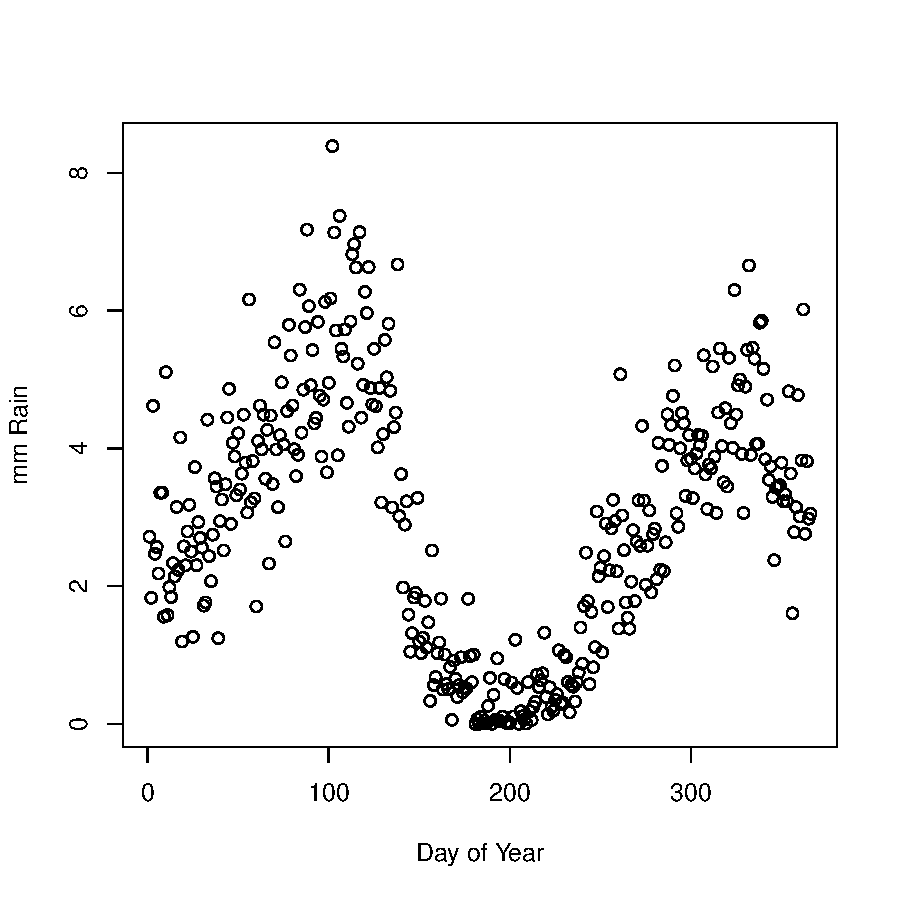
\includegraphics{climate_vignette-004}

Note the rainfall has two peaks, but does not fall to 0 in Dec/Jan.

\subsection{Markov Model}
The first thing we do is to add the Markov lags, up to order=2.

\begin{Schunk}
\begin{Sinput}
> zaza_wm=add_markov(zaza_doy)
> #load("zaza_wm")
> head(zaza_wm)
\end{Sinput}
\begin{Soutput}
  Station       Date Rain DOY wet_or_dry lag_1 lag_2
1    Zaza 1930-10-01    0 275          d  <NA>  <NA>
2    Zaza 1930-10-02    8 276          w     d  <NA>
3    Zaza 1930-10-03   43 277          w     w    wd
4    Zaza 1930-10-04    0 278          d     w    ww
5    Zaza 1930-10-05    0 279          d     d    dw
6    Zaza 1930-10-06   45 280          w     d    dd
\end{Soutput}
\end{Schunk}

Note there are three new columns.  "d" means a dry day and
"w" means any day in which the amount of rain is more than
some threshold (default 0.12 mm).  Lag\_n is the pattern
of wet and dry days over the previous n days.

We can now count for each day of year:the number of "w" days following
two "d" days; the number of "w" days following a "d" then a "w"
day etc.  Dividing by e.g. the number of times we have two consecutive
"d" days give the estimated probability.  The function {\tt make\_all\_probs}
does this, for all lags up to order  (default 2).
As well, for each day of year, we determine the mean and standard
deviation of the rain of a "w" day both unconditional, and conditioned
on lags up to {\tt max\_mean\_rain\_order} (default 1)

\begin{Schunk}
\begin{Sinput}
> #zaza_pbs=make_all_probs(zaza_wm)
> load("/home/william/Reading/rstudio/climate/zaza_pbs")
> head(zaza_pbs)
\end{Sinput}
\begin{Soutput}
  P(w) <rain> sd(rain) # days # wet days P(w|w) P(w|d) #w #d P(w|ww) P(w|dw)
1 0.29    9.4     16.0     62         18   0.30   0.27 20 41    0.17    0.38
2 0.34    5.4      7.9     62         21   0.50   0.27 18 44    0.50    0.43
3 0.52    8.9     13.0     62         32   0.71   0.41 21 41    0.89    0.56
4 0.27    9.0      8.2     62         17   0.38   0.17 32 30    0.53    0.33
5 0.39    6.6      7.1     62         24   0.65   0.29 17 45    0.67    0.35
6 0.40    5.4      7.9     62         25   0.58   0.29 24 38    0.55    0.33
  P(w|wd) P(w|dd) #ww #dw #wd #dd <(r|w)> <(r|d)> sd(r|w) sd(r|d) #rw #rd
1    0.50    0.20  12  16   8  25     2.0    12.7     2.4    19.5   6  11
2    0.55    0.20   6  14  11  30     4.3     6.2     5.3     9.6   9  12
3    0.58    0.38   9   9  12  32     7.7    10.1    13.1    13.2  15  17
4    0.24    0.12  15   6  17  24     9.7     7.4     9.3     4.8  12   5
5    0.60    0.24  12  20   5  25     3.8     9.0     3.7     8.5  11  13
6    0.62    0.28  11   6  13  32     3.2     8.2     3.8    10.6  14  11
\end{Soutput}
\end{Schunk}

As we can see from a plot, the probabilities are all over the map.

\begin{Schunk}
\begin{Sinput}
> plot(zaza_pbs[,"P(w|ww)"],xlab="Day of Year",ylab="P(w|ww)")
\end{Sinput}
\end{Schunk}
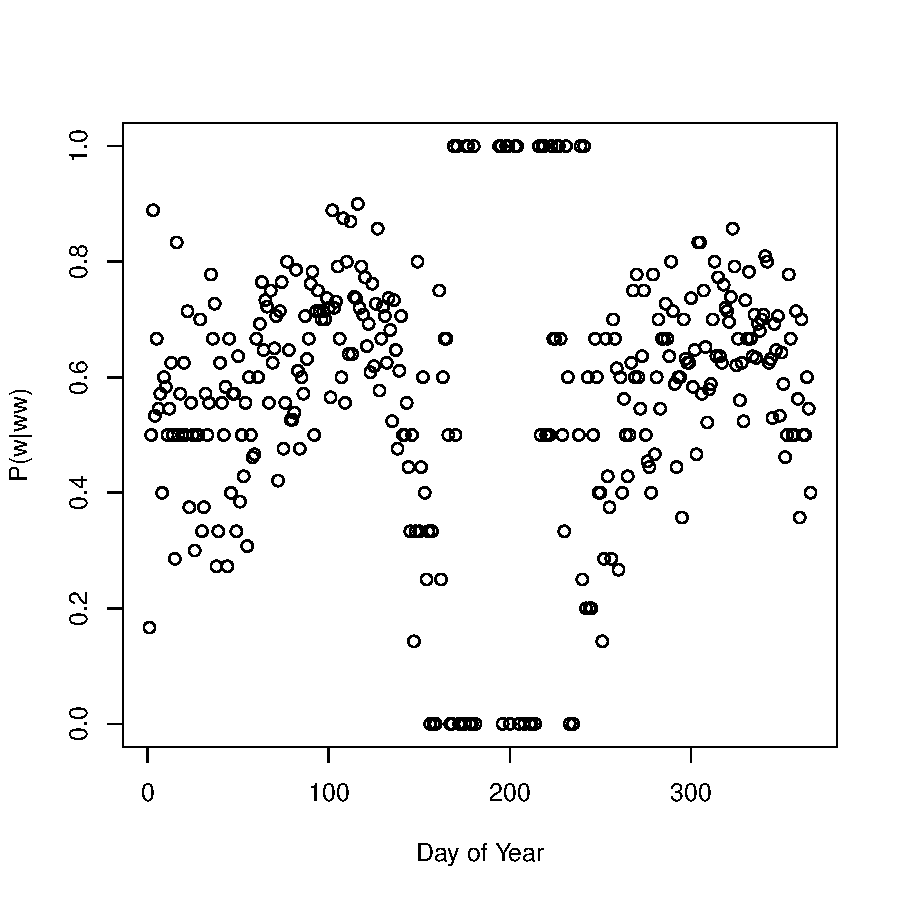
\includegraphics{climate_vignette-007}

This is due to the fact that the probabilities are based on
relatively few days.  Indeed for Jan 2, there were only 6
times when the previous two days were rainy.  However, we expect
that the probabilities on Jan 2 will be very similar to those
of Jan 3 and even something like the probabilities of Feb 4.
To achieve this we need to smooth the probabilities.  There are {\it many}
ways of doing this, the way used at present is to fit a Fourier series (this
has the advantage that we can make things periodic with period 1 year).
The order of the fit can be determined before hand or determined
interactively. The function used is {\tt make\_model\_ip}.

\subsection{Philosophy of Model}


\begin{Schunk}
\begin{Sinput}
>    zaza_mod = make_model_pl(zaza_pbs,"/home/william/Reading/rstudio/climate/trunk/inst/parameter/order_2_0.pl")
\end{Sinput}
\end{Schunk}


The basic idea of the package is to model
and analyze rainfall.
To determine the amount of rainfall on a given day
we use two steps.



\begin{enumerate}
\item  Get the probability that there will be rain.
\item  Get the distribution of the amount of rain on rainy days
\end{enumerate}

Central to the package is the {\tt model} data set.  
There are functions to create models (e.g. from known data)
and functions that use the model to create simulated
data.  There are also functions that analyze real or simulated
data.

This is an example of a model data set.   This
model was created from real data of the rainfall at
a site in Rwanda. The data set has 366 rows,
only the first 6 are shown

\begin{Schunk}
\begin{Sinput}
> head(zaza_mod)
\end{Sinput}
\begin{Soutput}
     info P(w|ww) P(w|dw) P(w|wd) P(w|dd) <rain> sd(rain)
[1,]    2    0.55    0.34    0.45    0.25    8.4      9.8
[2,]    2    0.55    0.34    0.45    0.25    8.4      9.8
[3,]    2    0.54    0.34    0.45    0.24    8.4      9.8
[4,]    0    0.54    0.34    0.45    0.24    8.4      9.8
[5,]    0    0.54    0.34    0.44    0.24    8.3      9.8
[6,]   NA    0.54    0.34    0.44    0.24    8.3      9.8
\end{Soutput}
\end{Schunk}

I will attempt to explain the model

The info column contains information about the model.
(note everything here can and probably will change)
The first number is the order of the probability
of rain markov model, the third number is the order
of the Amount of rain (in mm) markov model.



\subsubsection{Probability of Rain}

We use a markov model of order k of the probability of rain, that is the chance
of rain will depend on the pattern of wet and dry days over the
previous k days. The order can be chosen (standard is an order of two,
e.g in the given model)

If the order is k, then there are $2^k$ possible patterns of
wet, w, and dry, d,  days.  For $k=2$ we have ww, dw, wd, dd.  Note for
every pattern there is a column in the model called $P(w|\mbox{pattern})$
For each day (the rows 1--366) we have the probability applicable to that
day.  There is no restriction on where these values come from. They can
(as in this case) be fitted values from raw data, however there are other
possibities.

\subsubsection{Amount of rain}

We use a markov model of order k for both the mean and standard deviation
of the amount of rain.  Hence, the mean and standard deviation of the ammount
of rain
will depend of the pattern of wet and dry days over the previous
k days.  The order can be chosen (standard is an order of 1, or 0
(do not take into account any pattern))

If the order is k, then there are $2^k$ possible patterns of
wet, w, and dry, d,  days.  For $k=1$ we have w, d  Note for
every pattern there is a column in the model called $<(r|\mbox{pattern}>)$
and a column called $sd(r|\mbox{pattern})$
For each day (the rows 1--366) we have the mean or the standard deviation
There is no restriction on where these values come from.
Note we also have the $<\mbox{rain}>$ and $sd(\mbox{rain})$ columns.
These are the unconditional mean and standard devation of the rain
amount.

Note though there is a day of year dependence in the
model there is (as yet) no year dependence.

\subsubsection{Obtaining Values: shape, offset}


Each column, whether probability or amount is said to be a "curve".
As indicated, the model does not know where the curve came
from.  However, it is often usefull to break the curve down
into two parts.  a "shape" and an "offset".   The shape is
any general curve, the offset is a single number applied to the shape
to get the final curve.  So
\begin{equation}
\mbox(curve) = \mbox{shape} + \mbox{offset}
\end{equation}
(We do not attempt to make a canonical offset for the shape.
We need the weighted sum of squares fit to a constant to be zero,
but in practice the weighting is not known)

The motivation here, is that it is often noted that higher order
curves (eg $P(w|\mbox{dw})$ ) are often very similar to lower
order curves  (eg $P(w|\mbox{d})$ ) but with an offset.   Thus,
it makes sense to estimate the higher order curve
by estimating only this offset, rather than the large number
of parameters needed to directly estimate the higher order curve.

An example can help here.   We look at the same site that was
used to produce the above model.

\begin{figure}[H]
\centering
\includegraphics{/home/william/Reading/rstudio/climate/compare_1.jpeg}
\end{figure}

The blue line is the probability of rain given that the previous
day was dry, $P(w|\mbox{d})$.   This can be broken down into
$P(w|\mbox{dd})$, the red line, and $P(w|\mbox{dw})$, the green line.
We note that the green line has much the same shape as the
blue line but with a substantial offset.

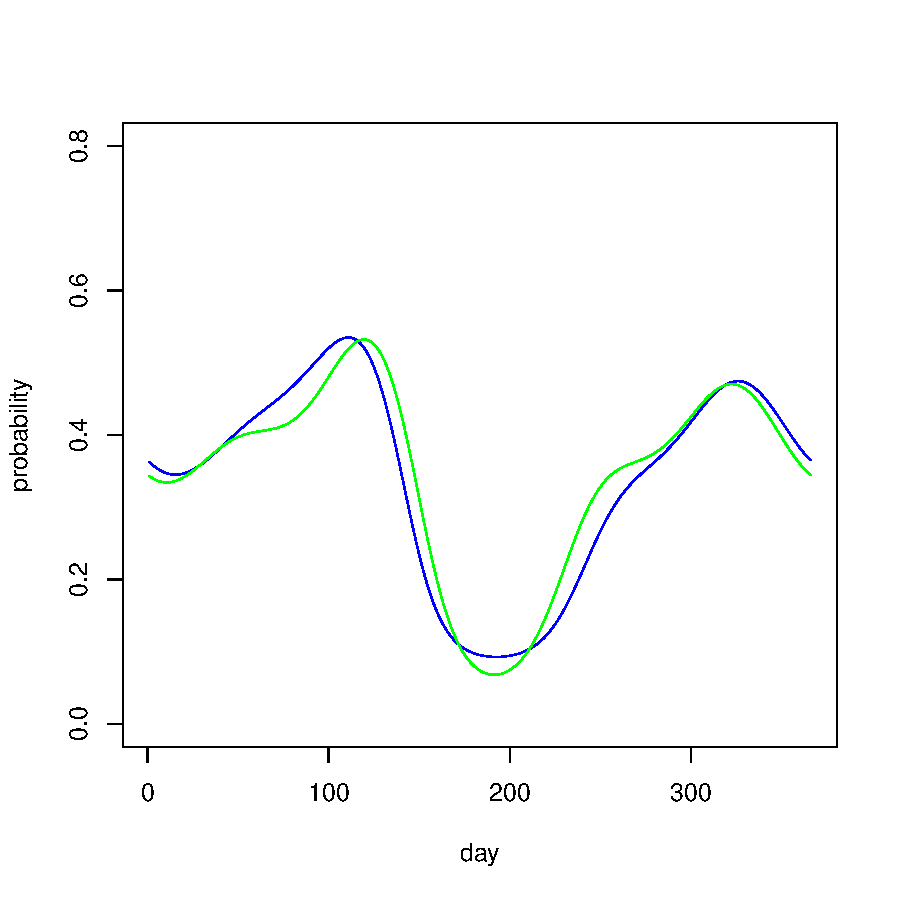
\includegraphics{climate_vignette-010}

Here we see $P(w|\mbox{d})$ (the blue line) shifted to match
$P(w|\mbox{dw})$ (the green line).  It seems that we can use
the shifted blue line rather than the green line.  Given that we have
much more confidence in the shifted blue line (more data, fewer coefficients)
that the green line, we may prefer to use the shifted blue line.

\section{Parameter Files and make\_model\_ip}

On way of creating a model is to start with a set of raw probabilities,
{\tt raw\_probs}, derived from a dataset associated (usually) with a station.
Then each curve $P(w|\mbox{lag})$ can be a fitted version of the corresponding
data in the dataset, or a (possibly shifted) fitted version of some other
data from the dataset.

The model is described by a {\tt parameter (*.pl)} file.
An example of the start of such a file is given.

\begin{verbatim}
<order> = 2
<dd> = dd  
<dd_fit_order>= choose
<dd_offset> = NO
...
\end{verbatim}

Every line has the form
\begin{verbatim}
<key> = value
\end{verbatim}
When read in you get a list, with {\tt list[key] = value}
with value a string.

The first parameter, {\tt order}, gives the order of the wet/dry part
of the model.  For each of the $2^{\mbox{order}}$ values for the {\tt lag},
there are three parameters.   The first {\tt lag} is the column
of the raw dataset used; the second {\tt lag\_fit\_order} is the number
of harmonics used to fit the raw data (if this value is {\tt choose} then the fit
order is determined automatically); the third {\tt lag\_offset}
is the dataset from which the offset is to be determined, if the
value is {\tt NO} then there is no offset.

The part of the parameter file which deals with the amount of rain on wet
days is similar,  although in this case we have {\tt lag} and {\tt lag\_sd}
for the mean and standard deviation.

\begin{verbatim}
<rain_order>= 1
<rw>=w
<rw_fit_order>=4
<rw_offset> = NO
<rw_sd>=w
<rw_sd_fit_order>=choose
<rw_sd_offset> = NO
...
\end{verbatim}

This is the "standard" parameter file, {\tt order\_2\_0.pl}.   It describes an order 2
model for the probability of rain, and an order zero model for the
amount of rain.

\begin{verbatim}
<order> = 2
<dd> = dd  
<dd_fit_order>= choose
<dd_offset> = NO
<dw> = dw
<dw_fit_order>= choose
<dw_offset> = NO
<wd>= wd
<wd_fit_order>= choose
<wd_offset> = NO
<ww> = ww
<ww_fit_order>= choose
<ww_offset> = NO

rain_order>= 0
<r0_fit_order>= 4
<r0_sd_fit_order>= 4

\end{verbatim}

If we want an order 1 model for the amount of rain, we change only
the rain section (last three line) to 

\begin{verbatim}
<rain_order>= 1
<rw>=w
<rw_fit_order>=4
<rw_offset> = NO
<rw_sd>=w
<rw_sd_fit_order>=4
<rw_sd_offset> = NO
<rd>=0
<rd_fit_order>=4
<rd_offset> = NO
<rd_sd>=0
<rd_sd_fit_order>=4
<rd_sd_offset> = NO
\end{verbatim}

We can get a mixed markov model by  changing what is used to estimate
higher order lags.

\begin{verbatim}
<order> = 2
<dd> = d  
<dd_fit_order>= choose
<dd_offset> = NO
<dw> = d
<dw_fit_order>= choose
<dw_offset> = NO
<wd>= wd
<wd_fit_order>= choose
<wd_offset> = NO
<ww> = ww
<ww_fit_order>= choose
<ww_offset> = NO


<rain_order>= 0
<r0_fit_order>= 4
<r0_sd_fit_order>= 4
\end{verbatim}

Note that the curves for the order two lags dd and dw are both derived 
from the order 1 curve lag d.  However the curves for the order 2
lags wd and ww are derived from order two curves.  In other words we only
use order 2 lags if the first day is wet.

We can add offsets if desired.  Let us change the offset for the curve
for lag dw.

\begin{verbatim}
<dw> = d
<dw_fit_order>= choose
<dw_offset> = dw
\end{verbatim}

Note that we still derive the curve from the first order lag,
but now we add an offset derived from the second order lag.

We can illustrate this by using the above data set.
(here we are looking a only the probability of rain)

First we show a second order model

\begin{Schunk}
\begin{Sinput}
> mod=make_model_pl(zaza_pbs,"/home/william/Reading/rstudio/climate/trunk/inst/parameter/order_2_0.pl")
> plot_model(mod,"Second Order Model")
\end{Sinput}
\end{Schunk}
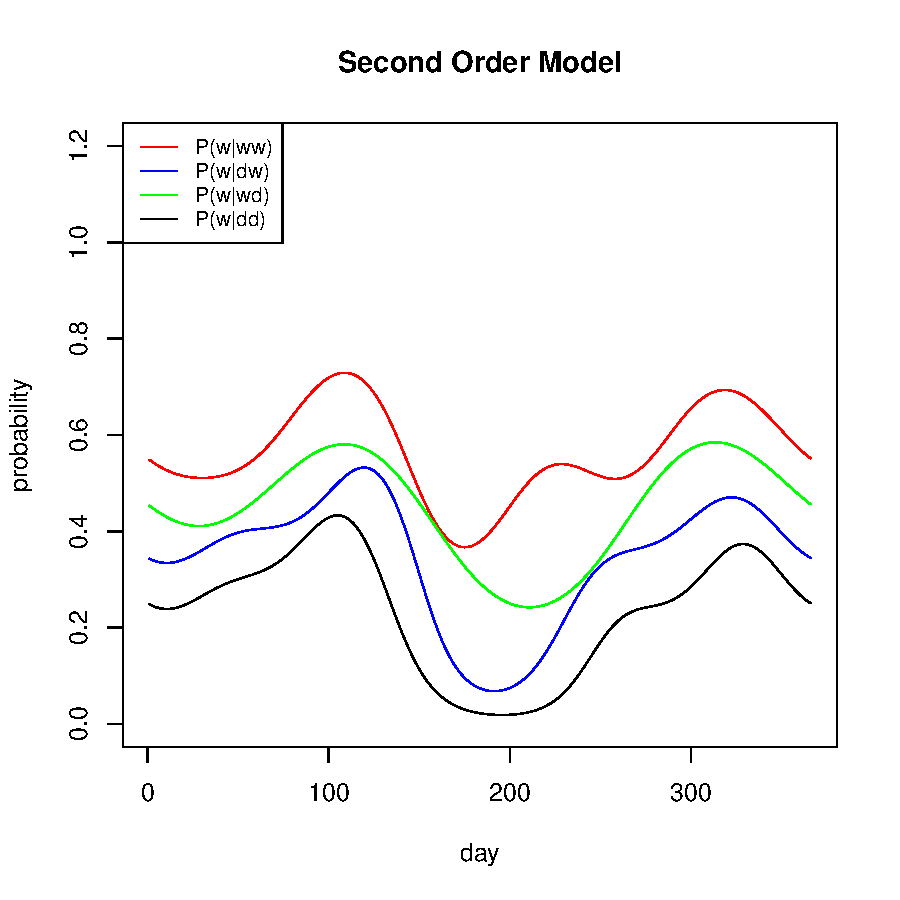
\includegraphics{climate_vignette-011}

As we have noted above, the wd, and ww, lines are not close
in shape to the w line, but the dd and dw lines are close in
shape to the d line.   So we can try a mixed model, going
to order 2 lags if the previous day was wet, but using only
order 1 if the previous day was dry

\begin{Schunk}
\begin{Sinput}
> mod=make_model_pl(zaza_pbs,"/home/william/Reading/rstudio/climate/trunk/inst/parameter/order_2_(2_1)_0.pl")
> plot_model(mod,"Mixed Model (wet 2, dry 1) ")
\end{Sinput}
\end{Schunk}
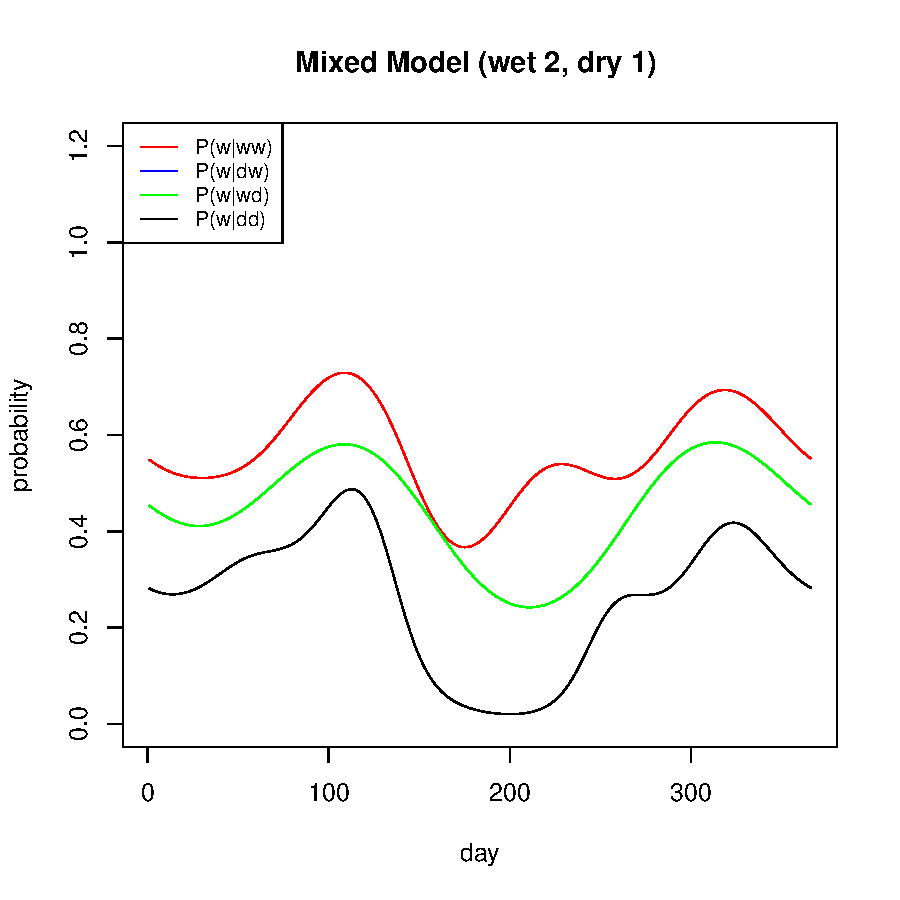
\includegraphics{climate_vignette-012}

Note that {\tt P(w|dw)} and {\tt P(w|dd)} are identical.  The latter
obscures the former.

We note from above that the d line can be used for dd
but while the dw line is similar in shape to dd there is an
obvious offset.   We can include this offset.

\begin{Schunk}
\begin{Sinput}
> mod=make_model_pl(zaza_pbs,"/home/william/Reading/rstudio/climate/trunk/inst/parameter/offset.pl")
> plot_model(mod,"Mixed Model (wet 2, dry 1) dw offset")
\end{Sinput}
\end{Schunk}
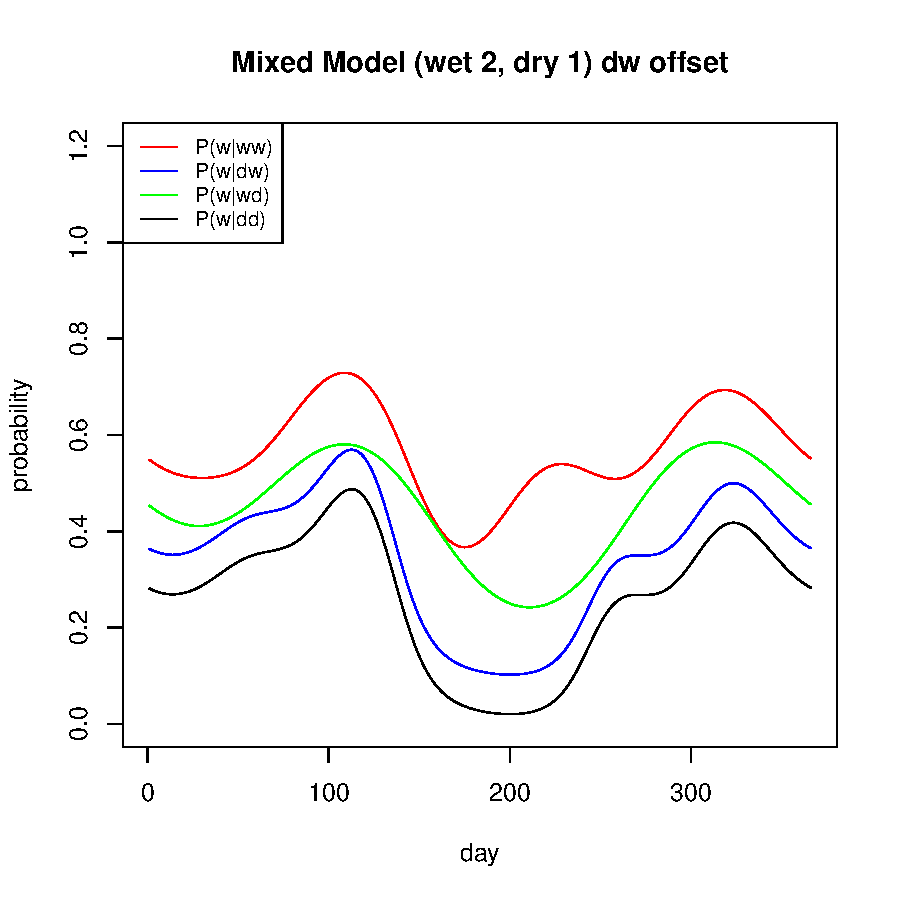
\includegraphics{climate_vignette-013}


\subsection{smoothing}


When fitting to obtain the model , we weight each estimate by the number of observations used to
obtain the estimate.  So estimates based on only a single day (e.g. two
consecutive "w" days during the dry season) are not given much weight.   

\begin{Schunk}
\begin{Sinput}
> plot(zaza_mod[,"P(w|ww)"],xlab="Day of Year",ylab="P(w|ww)")
\end{Sinput}
\end{Schunk}
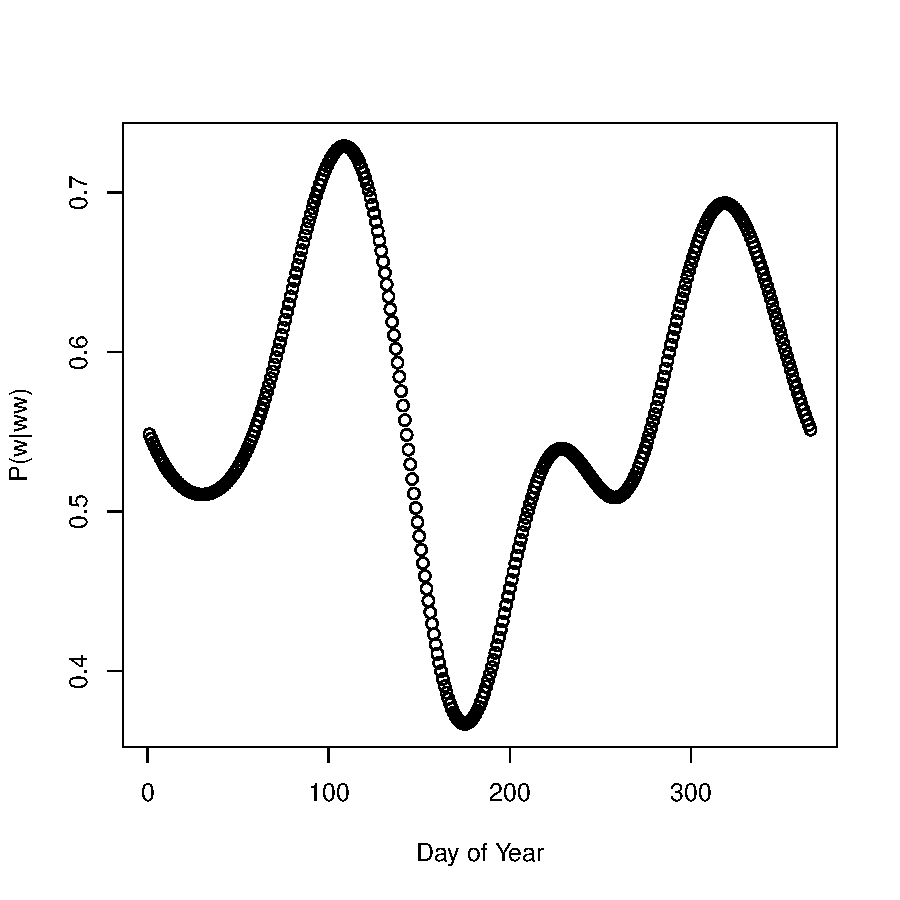
\includegraphics{climate_vignette-014}

And things look much smoother.   


We can also do the fitting interactively.  At the console, enter the command
\begin{Schunk}
\begin{Sinput}
> zaza_mod = make_model_general(zaza_pbs,inter=TRUE)
\end{Sinput}
\end{Schunk}
We see a graph 

\begin{figure}[h!]
\centering
\includegraphics{/home/william/Reading/rstudio/climate/inter_plot1.jpeg}
\end{figure}

The red circles represent data points.  The are of each circle is proportional
to the weighting the data point has in the fit.  The smallest circles are
data point calculated from a single line of the raw data 
(so for probabilities are 0 or 1).

The blue line represents the fitted curve.  It will change when we change
the order of the Fourier fit.

On the console you will see:

\begin{figure}[h!]
\centering
\begin{verbatim}
enter

a:  use this fit
b:  use previous order
f:  add one to order
k:  set order to k
\end{verbatim}
\end{figure}
To enter a value you must type the value into the console and then press
return.  Entering a number changes the fit order to that number.  Try entering
8.  You get:

\begin{figure}[H]
\centering
\includegraphics{/home/william/Reading/rstudio/climate/inter_plot2.jpeg}
\end{figure}

The fit does not look that much better, especially when considering
how much more wavy the line is.  Try entering 1.  You get:

\begin{figure}[H]
\centering
\includegraphics{/home/william/Reading/rstudio/climate/inter_plot3.jpeg}
\end{figure}


Clearly we are now underfitting.   Enter 4, to get back to the first graph,
then enter {\tt a} to accept this fit.  You will then have 5 more graphs
to fit. Play around with the {\tt a,b} and {\tt f} keys or enter numbers.
Repeatedly pressing {\tt a} will use the default.

\subsection{Synthetic Data}

Once we have a model, we can use it to synthesize data.  The command is

\begin{Schunk}
\begin{Sinput}
> #load("zaza_synth")
> zaza_synth=synth_data_set_mod(zaza_mod,num_years=83)
> head(zaza_synth)
\end{Sinput}
\begin{Soutput}
  Station       Date  Rain DOY
1   synth 1970-01-01  0.00   1
2   synth 1970-01-02  0.18   2
3   synth 1970-01-03 14.48   3
4   synth 1970-01-04 23.71   4
5   synth 1970-01-05  0.67   5
6   synth 1970-01-06 29.14   6
\end{Soutput}
\end{Schunk}
The data will start from year 1970 by default.  The number
of years produced is limited by your patience (and by the address space of your
machine,  200,000 years for a 32 bit machine; you need to have a {\bf LOT} of patience to reach the limit if you 
have a 64 bit machine).
As a rule of thumb 1000 years takes about a minute (your mileage will vary).

Let's compare the synthetic and the real data.  Clearly we cannot expect
day by day comparisons to be equal, indeed, compare the rain in 1931, to the first year of rain in the synthetic data.

\begin{Schunk}
\begin{Sinput}
> plot(zaza$Rain[93:459],xlab="Day of Year",ylab="mm Rain")
> points(zaza_synth$Rain[1:366],col="green")
\end{Sinput}
\end{Schunk}
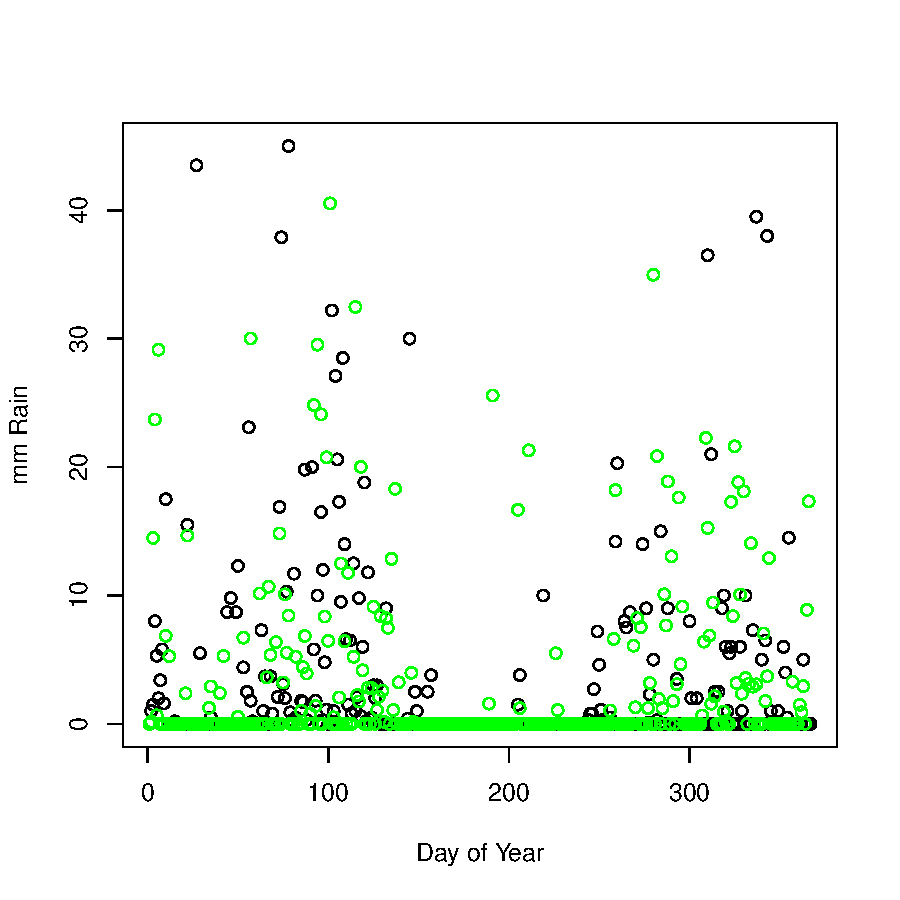
\includegraphics{climate_vignette-017}

The exact values are different, but the pattern is similar.
We now take advantage of the r function {\tt x\_split=split(x,y)}
where x and y are in the same dataframe.  What this gives is a list
indexed by the values of y.  Each element contains every value
of x with the given value of y.  So {zaza\_split=split(zaza\_doy$Rain,zaza\_doy$DOY)}
is a list of 366 vectors. {\\tt zaza\_split[["120"]]} is a vector of all rainfall
on Day of Year 120.  So {\tt mean(zaza\_split[["120"]],na.rm=TRUE)} is the mean
rainfall on day 120 (the last arg means ignore NA's).  We take further advantage by using the r function {\tt sapply(list, function,args)} which applies  function
to every element of list, passing args to function.  So
{\tt sapply(zaza\_split,mean,na.rm=TRUE)} is a vector of the average rainfalls.
Comparing

\begin{Schunk}
\begin{Sinput}
> zaza_split=split(zaza_doy$Rain,zaza_doy$DOY)
> synth_split=split(zaza_synth$Rain,zaza_synth$DOY)
> plot(sapply(zaza_split,mean,na.rm=TRUE),xlab="Day of Year",
+      ylab="Average Rain mm.")
> points(sapply(synth_split,mean,na.rm=TRUE),col="green")
\end{Sinput}
\end{Schunk}
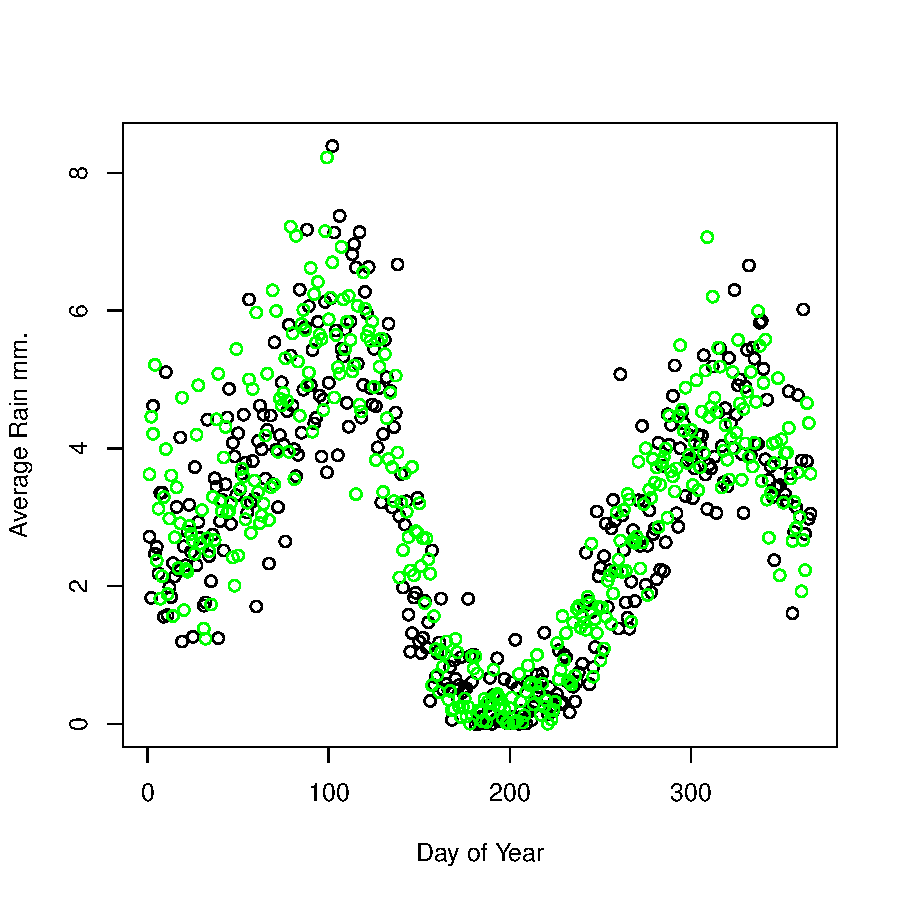
\includegraphics{climate_vignette-018}

The fit looks good.
\subsection{Yearly Stats}

If we split our real or synthetic data set by {\tt mod\_year}
then we get a list of datasets, each covering a specific year. We can then
find things such a the average spell length (over years), the maximum dry spell
for each year etc.  There is a simple function to split by {\tt mod\_year}
adding it if it does not exist.  The function {\tt add\_spell\_info} calculates
and adds the length of wet and dry spells.
This should be applied before splitting if spells should cross year boundaries.
Note that we need to add the Markov stuff before adding spell info.

\begin{Schunk}
\begin{Sinput}
> synth_wm= add_markov(zaza_synth)
> synth_spell= add_spell_info(synth_wm)
> zaza_spell=add_spell_info(zaza_wm)
> synth_split=split_by_year(synth_spell,year_begins_in_july=TRUE)
> zaza_split=split_by_year(zaza_spell,year_begins_in_july=TRUE)
> length(synth_split)
\end{Sinput}
\begin{Soutput}
[1] 84
\end{Soutput}
\begin{Sinput}
> head(synth_split[["1981"]])
\end{Sinput}
\begin{Soutput}
     Station       Date Rain DOY wet_or_dry lag_1 lag_2 first_DOY spell_length
3843   synth 1980-07-01    0 183          d     d    dd       178           22
3844   synth 1980-07-02    0 184          d     d    dd       178           22
3845   synth 1980-07-03    0 185          d     d    dd       178           22
3846   synth 1980-07-04    0 186          d     d    dd       178           22
3847   synth 1980-07-05    0 187          d     d    dd       178           22
3848   synth 1980-07-06    0 188          d     d    dd       178           22
     mod_year month day
3843     1981     7   1
3844     1981     7   2
3845     1981     7   3
3846     1981     7   4
3847     1981     7   5
3848     1981     7   6
\end{Soutput}
\begin{Sinput}
> nrow(synth_split[["1981"]])
\end{Sinput}
\begin{Soutput}
[1] 366
\end{Soutput}
\begin{Sinput}
> length(zaza_split)
\end{Sinput}
\begin{Soutput}
[1] 82
\end{Soutput}
\begin{Sinput}
> head(zaza_split[["1951"]])
\end{Sinput}
\begin{Soutput}
     Station       Date Rain DOY wet_or_dry lag_1 lag_2 first_DOY spell_length
7229    Zaza 1950-07-01    0 183          d     d    dd       151           89
7230    Zaza 1950-07-02    0 184          d     d    dd       151           89
7231    Zaza 1950-07-03    0 185          d     d    dd       151           89
7232    Zaza 1950-07-04    0 186          d     d    dd       151           89
7233    Zaza 1950-07-05    0 187          d     d    dd       151           89
7234    Zaza 1950-07-06    0 188          d     d    dd       151           89
     mod_year month day
7229     1951     7   1
7230     1951     7   2
7231     1951     7   3
7232     1951     7   4
7233     1951     7   5
7234     1951     7   6
\end{Soutput}
\begin{Sinput}
> nrow(zaza_split[["1951"]])
\end{Sinput}
\begin{Soutput}
[1] 366
\end{Soutput}
\end{Schunk}

So  {\tt synth\_split} consists of 84 data sets (there is a partial
year at the beginning and end) and {\tt zaza\_split}
consists of 82 data sets (there are no partial years.)

\subsubsection{Spell Lengths}

We can look at the average dry spell length.  For this we use the data
that has not been spit into years.  First we take only dry spells.
To do this, take only rows of {\tt zaza\_spell} that correspond to a dry
day.  

\begin{Schunk}
\begin{Sinput}
> zaza_dry=zaza_spell[(zaza_spell$wet_or_dry=="d"),]
> head(zaza_dry)
\end{Sinput}
\begin{Soutput}
  Station       Date Rain DOY wet_or_dry lag_1 lag_2 first_DOY spell_length
1    Zaza 1930-10-01    0 275          d  <NA>  <NA>       275            1
4    Zaza 1930-10-04    0 278          d     w    ww       278            2
5    Zaza 1930-10-05    0 279          d     d    dw       278            2
7    Zaza 1930-10-07    0 281          d     w    wd       281            4
8    Zaza 1930-10-08    0 282          d     d    dw       281            4
9    Zaza 1930-10-09    0 283          d     d    dd       281            4
\end{Soutput}
\end{Schunk}

Now we split the spell lengths by day of year, 
then take the mean (ignoring NA's).  Plot this

\begin{Schunk}
\begin{Sinput}
> dry_spell_split=split(zaza_dry$spell_length,zaza_dry$DOY)
> plot(sapply(dry_spell_split,mean,rm.na=T),type="l",xlab="Day of Year",
+      ylab="Days",main="Mean Length of Dry Spell")
\end{Sinput}
\end{Schunk}
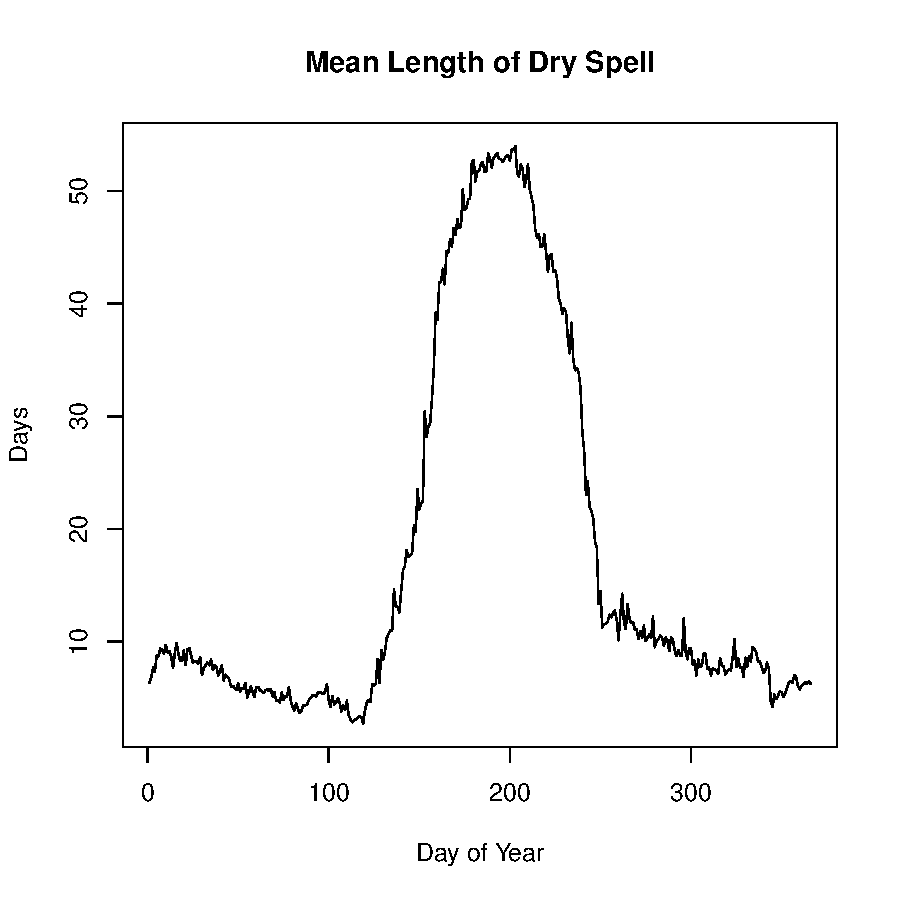
\includegraphics{climate_vignette-021}

Note this is the average length of a dry spell, given that there
is a dry spell.  This may or may not be what you want.  If you want
the mean dry spell length, taking the dry spell length of a wet day
to be 0 then this can be done by adding another column.

\begin{Schunk}
\begin{Sinput}
> zaza_spell$dry_spell_length=zaza_spell$spell_length
> zaza_spell$dry_spell_length[zaza_spell$wet_or_dry == "w"]=0
> zaza_spell$dry_spell_length[is.na(zaza_spell$wet_or_dry)]=NA
> zaza_spell_dry_split=split(zaza_spell$dry_spell_length,zaza_spell$DOY)
> plot(sapply(zaza_spell_dry_split,mean,na.rm=T),type="l")
\end{Sinput}
\end{Schunk}
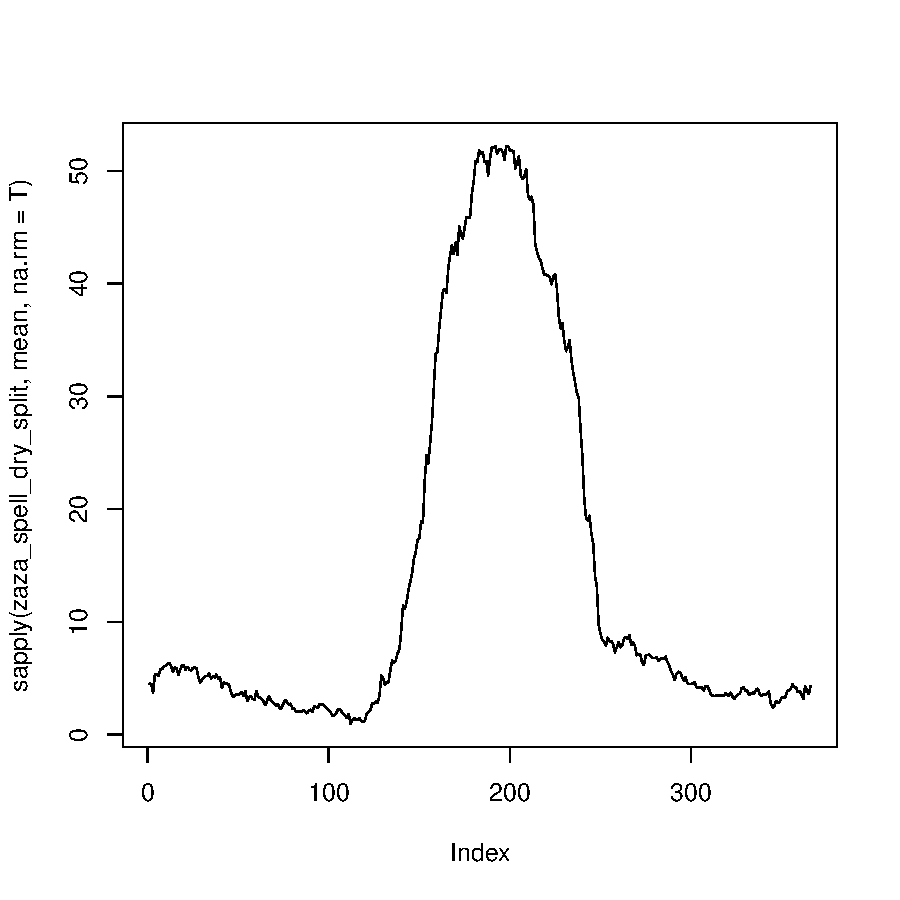
\includegraphics{climate_vignette-022}
This looks similar.  Plot them together for comparison.  (note the use of
the {\tt lines} function which adds lines to a graph)

\begin{Schunk}
\begin{Sinput}
> plot(sapply(dry_spell_split,mean,rm.na=T),type="l",xlab="Day of Year",
+      ylab="Days",main="Mean Length of Dry Spell")
> lines(sapply(zaza_spell_dry_split,mean,na.rm=T),col="green")
\end{Sinput}
\end{Schunk}
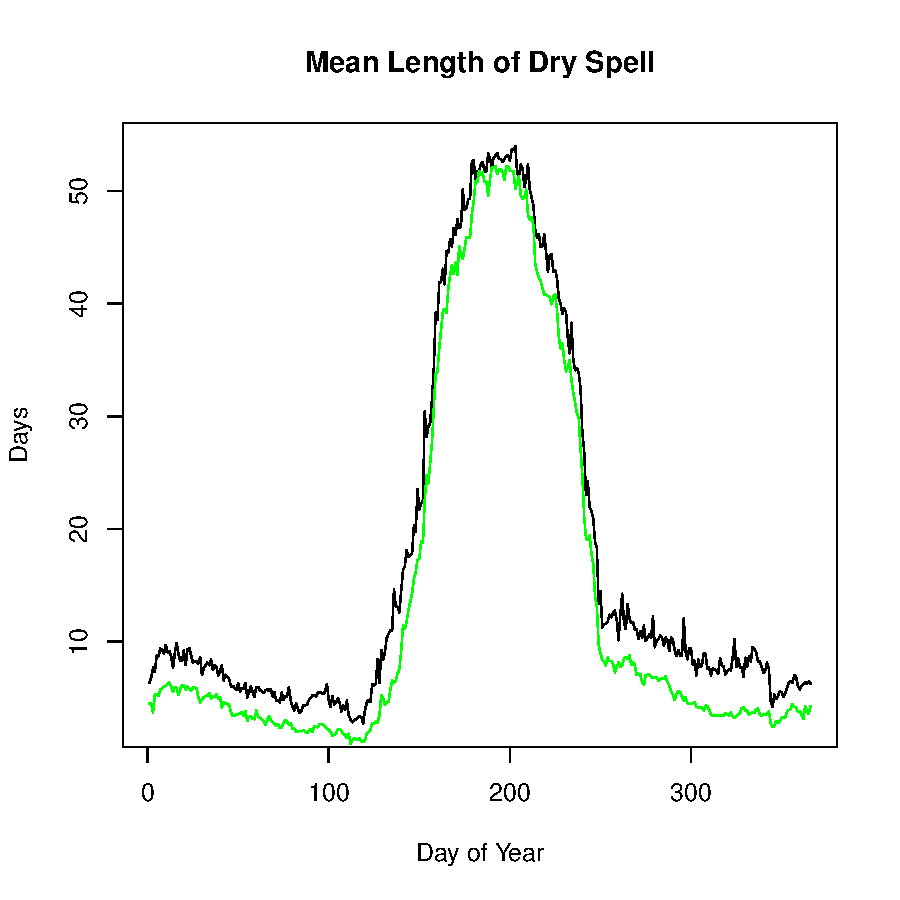
\includegraphics{climate_vignette-023}

Assume that we know our crop can withstand dry spells of up to 
5 days.  Then we are interested in the probability of a dry spell
of more than 5 days.  

\begin{Schunk}
\begin{Sinput}
> zaza_dry_spell_over_5=zaza_spell[zaza_spell$wet_or_dry=="d" & zaza_spell$spell_length > 5,]
> zaza_dry_spell_over_5_split=split(zaza_dry_spell_over_5,zaza_dry_spell_over_5$DOY)
> num_of_dry_spells_over_5=sapply(zaza_dry_spell_over_5_split,nrow)
> zaza_spell_good=zaza_spell[!is.na(zaza_spell$wet_or_dry),]
> zaza_spell_good_split=split(zaza_spell_good,zaza_spell_good$DOY)
> num_good_days=sapply(zaza_spell_good_split,nrow)
> prob_of_dry_spell_over_5=num_of_dry_spells_over_5/num_good_days
> plot(prob_of_dry_spell_over_5,type="l",xlab="Day of Year",ylab="prob",
+        main="Probability of a dry spell of more than 5 days")
\end{Sinput}
\end{Schunk}
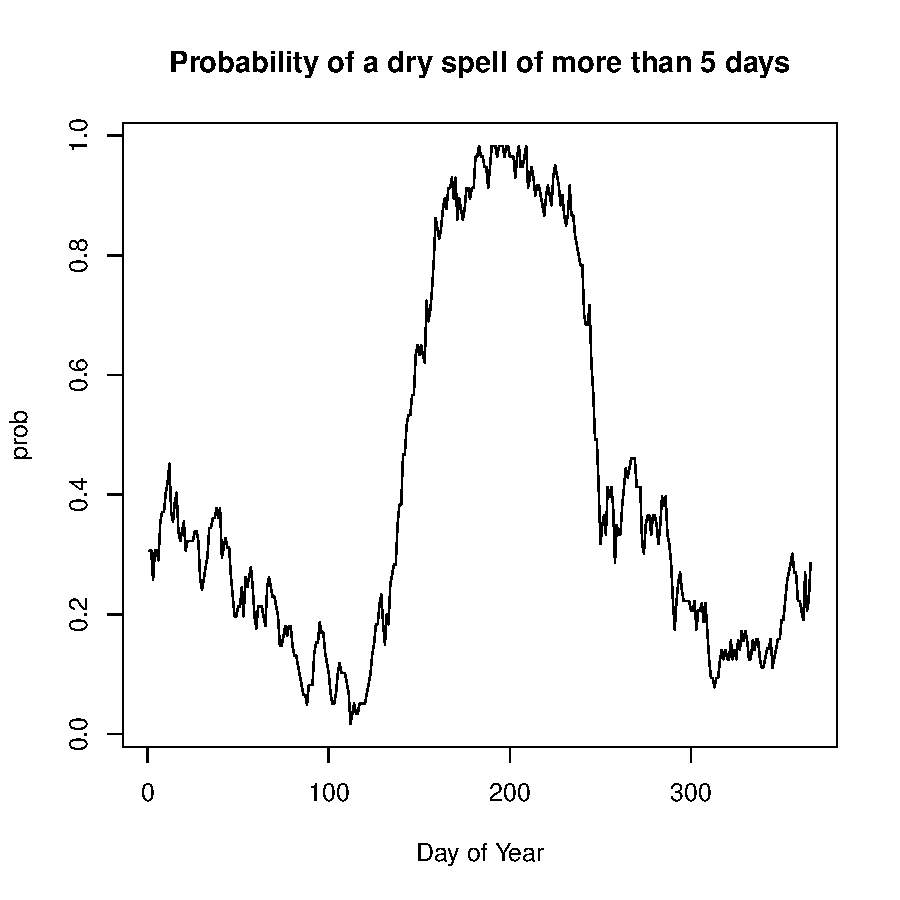
\includegraphics{climate_vignette-024}

Naturally, all the above can be done with synthetic data as well.
(Indeed, this is the whole point.  Get your model from 20 years of
real data, but get your probabilities from 100 or 1000 years of
synthesized data.  In some cases, the actual value can be obtained
from the model by clever analysis (e.g. Markov model's and spell probabilities). 
However, R is cheap and fast; Statisticians capable of doing the analyses
are expensive and slow.  And what happens when you modify your
model?)

\subsubsection{First Day of Growing Season}

Two common definitions of the "First Day of the Growing Season" are:

\begin{enumerate}
\item  The first day of a period of n rainy days on which there is more than k
millimetres of rain in total
\item  As (1.) but additionally, there is no dry spell of k days in the next
j days
\end{enumerate}

The second definition may be defined as the time of successful planting
(young seedlings may be injured or killed by a dry spell of k days)
The function {\tt fdgs} can calculate either of these for a year
of data.  So if we apply it to every year of data to find the distribution
of the "First Day of the Growing Season"  (we start our search in July
if the growing season occurs in "winter").  So:

\begin{Schunk}
\begin{Sinput}
> first_days=sapply(zaza_split,fdgs)
> first_days_succ=sapply(zaza_split,fdgs,type=2)
\end{Sinput}
\end{Schunk}

and we can do the same thing with synthetic data

\begin{Schunk}
\begin{Sinput}
> first_days_synth=sapply(synth_split,fdgs)
> first_days_succ_synth=sapply(synth_split,fdgs,type=2)
\end{Sinput}
\end{Schunk}

In this case a histogram is best for viewing a comparison.

\begin{Schunk}
\begin{Sinput}
> hist(first_days,breaks=25,col="red",density=10,
+      xlab="Day of Year",main="First Day of Growing Season")
\end{Sinput}
\end{Schunk}
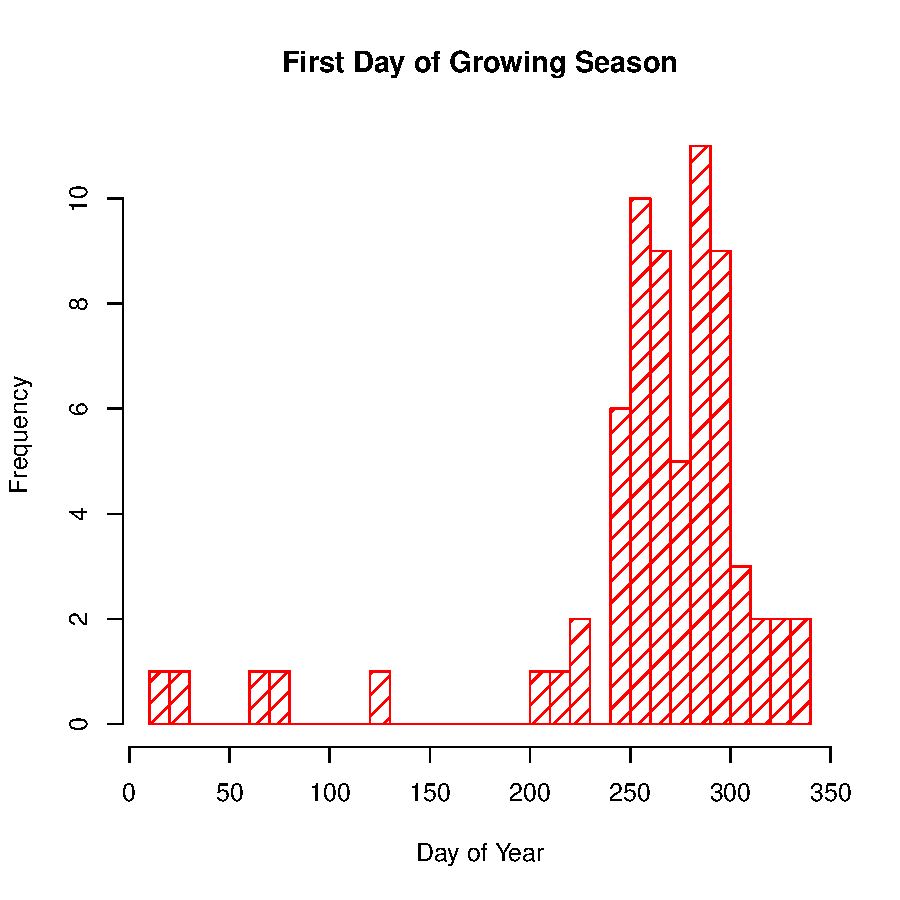
\includegraphics{climate_vignette-027}
We can compare this with the calculations from the synthetic data
(note for adding information to a histogram, use the {\tt add=T})
parameter.

\begin{Schunk}
\begin{Sinput}
> hist(first_days,breaks=25,col="red",density=10,
+      xlab="Day of Year",main="First Day of Growing Season")
> hist(first_days_synth,breaks=25,col="green",density=5,add=T)
\end{Sinput}
\end{Schunk}
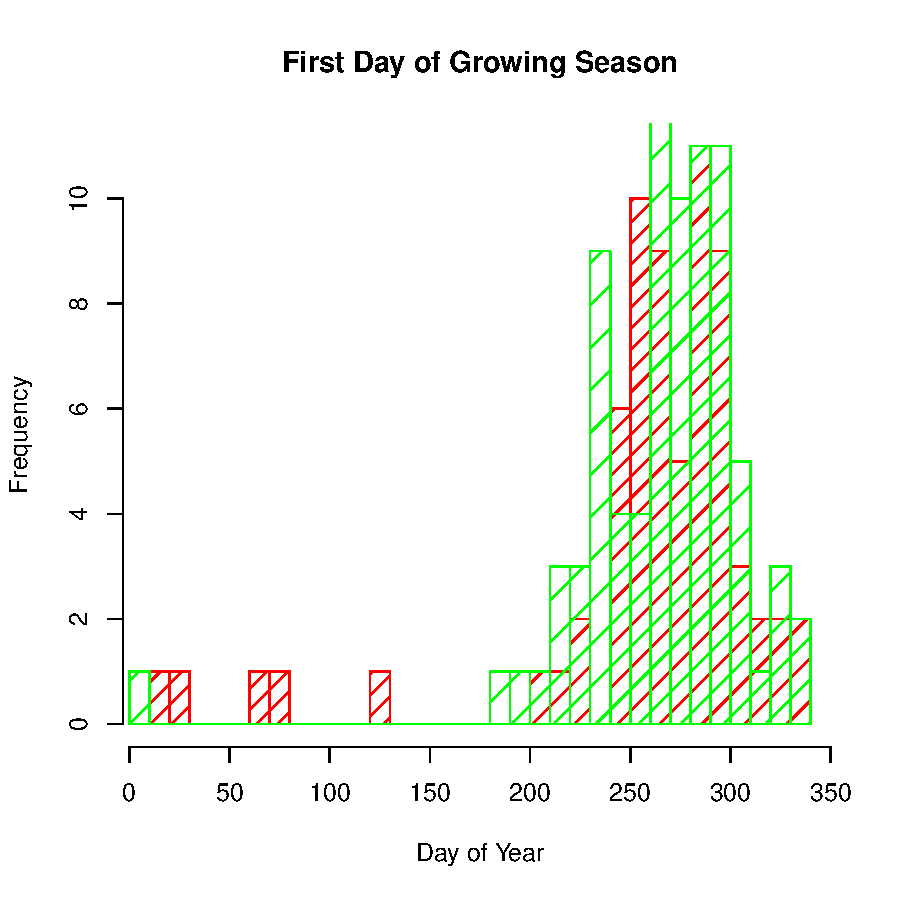
\includegraphics{climate_vignette-028}

Again, this is similar but not identical.

Another question we might ask is:  "In how many of the 82 years
was planting by definition 1. successful?"
To answer this we can compare, {\tt first\_days}
and {\tt first\_days\_succ}.  We need to be careful to allow
for NA's and for modding by 366.

\begin{Schunk}
\begin{Sinput}
> diff=(first_days_succ-first_days) %% 366
> diff_no_na=diff[!is.na(diff)]
> diff_good=diff_no_na[diff_no_na==0]
> length(diff_good)/length(diff_no_na)
\end{Sinput}
\begin{Soutput}
[1] 0.51
\end{Soutput}
\end{Schunk}

This suggests that the default values do not work
well for this site. Perhaps a more drought tolerant crop
would work better, or wait for more rain before saying
the growing season has started.

\section{Mixed order Markov Models}

<while this section is still accurate in that {\tt make\_model\_general}
sill exists and works, the functionality of {\tt make\_model\_general}
is not in the more general {\tt make\_model\_pl}.  The theoretical
stuff is still applicable.>

Examination of the different fits shows that the order needed in the markov
model can vary for different patterns of wet and dry days.  E.g.  It may
be that the probability of a wet day given that the previous day was wet
is not different if it was wet two days ago or if it was dry two days ago.
However, at the same time, it may be that the probability of a wet day, given
that the previous day was dry does depend on whether it was wet or dry two
days ago.  In symbols
\begin{equation}
P(w|wd)=P(w|ww)=P(w|w)
\end{equation}
but
\begin{equation}
P(w|dd) \neq P(w|dw) \neq P(w|d)
\end{equation}

To handle these type of cases a mixed markov model, has been created.
This is just a list, the first element is the order. (This is the maximum
of the order for wet days and dry days) There
follow $2^{\mbox{order}}$ strings, each named for one of the
possible lag patterns.  To use the model you simply index by the lag
pattern and the model will tell you which lag to actually use.
E.g. Let m be the mixed markov model for the above case.
We have
\begin{equation}
m[1]=2, m["wd"]="w", m["ww"]="w", m["dw"]="dw", m["dd"]="dd"
\end{equation}
The model is characterized by two variables {\tt max\_w\_order} and
{\tt max\_d\_order}.  In the above case these have the values 1 and 2
respectively.  Similarly, there are two variables {\tt max\_rain\_w\_order}
{\tt max\_rain\_d\_order}, which deal with, not if there is going to be rain,
but the mean and standard deviation of the amount of rain, given that
the day is wet.  

All variables are parameters to the function {\tt make\_model\_general}.
The values are stored as part of the model produced.  To use this function
you must first call {\tt make\_all\_probs} which requires a data set with
markov lags added by {\tt add\_markov}.  Both of these functions take
one or more order parameters.  If these orders are less that the highest
order used by {\tt make\_model\_general} the function will fail.
As an example

\begin{Schunk}
\begin{Sinput}
> #load("zaza_wm_3")
> zaza_wm_3=add_markov(zaza_doy,order=3)
> #load("zaza_all_pbs")
> zaza_all_pbs=make_all_probs(zaza_wm_3,max_rainy_day_order=3,
+                             max_mean_rain_order=2)
> head(zaza_all_pbs)
\end{Sinput}
\begin{Soutput}
  P(w) <rain> sd(rain) # days # wet days P(w|w) P(w|d) #w #d P(w|ww) P(w|dw)
1 0.29    9.4     16.0     62         18   0.30   0.27 20 41    0.17    0.38
2 0.34    5.4      7.9     62         21   0.50   0.27 18 44    0.50    0.43
3 0.52    8.9     13.0     62         32   0.71   0.41 21 41    0.89    0.56
4 0.27    9.0      8.2     62         17   0.38   0.17 32 30    0.53    0.33
5 0.39    6.6      7.1     62         24   0.65   0.29 17 45    0.67    0.35
6 0.40    5.4      7.9     62         25   0.58   0.29 24 38    0.55    0.33
  P(w|wd) P(w|dd) #ww #dw #wd #dd P(w|www) P(w|dww) P(w|wdw) P(w|ddw) P(w|wwd)
1    0.50    0.20  12  16   8  25     0.17     0.44     0.50     0.00     0.17
2    0.55    0.20   6  14  11  30     0.50     0.30     0.83     0.20     0.50
3    0.58    0.38   9   9  12  32     0.67     1.00     0.83     0.25     1.00
4    0.24    0.12  15   6  17  24     0.50     0.00     0.20     0.00     0.57
5    0.60    0.24  12  20   5  25     0.88     0.43     0.50     0.00     0.25
6    0.62    0.28  11   6  13  32     0.62     0.50     0.71     0.23     0.33
  P(w|dwd) P(w|wdd) P(w|ddd) #www #dww #wdw #ddw #wwd #dwd #wdd #ddd <(r|w)>
1     0.29     0.50     0.25    6    9    4    5    6    7    4   20     2.0
2     0.75     0.20     0.20    2   10    6   10    4    4    5   20     4.3
3     0.40     0.33     0.42    3    3    6    8    6    5    6   24     7.7
4     0.40     0.25     0.15    8    1    5    4    7    5   12   20     9.7
5     0.31     0.67     0.29    8    7    2    4    4   13    3   21     3.8
6     0.00     0.50     0.32    8    4    7   13    3    2    6   19     3.2
  <(r|d)> sd(r|w) sd(r|d) #rw #rd <(r|ww)> <(r|dw)> <(r|wd)> <(r|dd)> sd(r|ww)
1    12.7     2.4    19.5   6  11      4.2      5.0      1.0     22.0     3.61
2     6.2     5.3     9.6   9  12      5.3      8.8      3.8      3.6     7.33
3    10.1    13.1    13.2  15  17      4.2     10.8     11.7      9.7     3.64
4     7.4     9.3     4.8  12   5      9.6     12.2      9.9      4.1    10.60
5     9.0     3.7     8.5  11  13      3.1     10.6      5.6      7.2     3.13
6     8.2     3.8    10.6  14  11      1.4      6.1      4.5      8.7     0.87
  sd(r|dw) sd(r|wd) sd(r|dd) #rww #rdw #rwd #rdd
1      4.0     0.73     27.1    2    6    4    5
2     13.1     4.79      3.7    3    6    6    6
3      9.3    18.71     14.9    8    5    7   12
4      3.0     7.50      1.4    8    2    4    3
5      8.6     5.22      8.7    8    7    3    6
6      2.7     4.70     11.8    6    2    8    9
\end{Soutput}
\begin{Sinput}
> zaza_mod=make_model_general(zaza_all_pbs,max_w_order=1,max_d_order=3,
+                             max_rain_w_order=1, max_rain_d_order=2)
> head(zaza_mod)
\end{Sinput}
\begin{Soutput}
     info P(w|w) P(w|dww) P(w|ddw) P(w|dwd) P(w|ddd)          <rain> sd(rain)
[1,]    3   0.49     0.41     0.26     0.29     0.26 NA NA NA     NA       NA
[2,]    1   0.49     0.40     0.27     0.29     0.26 NA NA NA     NA       NA
[3,]    3   0.48     0.40     0.27     0.29     0.26 NA NA NA     NA       NA
[4,]    1   0.48     0.40     0.27     0.29     0.25 NA NA NA     NA       NA
[5,]    2   0.47     0.40     0.27     0.29     0.25 NA NA NA     NA       NA
[6,]   NA   0.47     0.39     0.27     0.29     0.25 NA NA NA     NA       NA
     <(r|w)> sd(r|w) <(r|dw)> sd(r|dw) <(r|dd)> sd(r|dd)
[1,]     7.7     8.6      8.6      8.0      9.3      9.6
[2,]     7.7     8.5      8.6      8.0      9.3      9.6
[3,]     7.6     8.4      8.6      8.1      9.3      9.6
[4,]     7.6     8.4      8.6      8.1      9.3      9.6
[5,]     7.5     8.3      8.6      8.2      9.3      9.7
[6,]     7.5     8.3      8.6      8.2      9.3      9.7
\end{Soutput}
\end{Schunk}

The model, {\tt zaza\_mod}, uses a lag of 1 for wet days and
a lag of 3 for dry days.  So if the previous day was wet, then the 
probability that today will be wet does not depend on what happened
before this.  On the other hand if the previous day was dry, then the
probability that today will be wet depends on what happened two days
ago and three days ago.  Similarly, if the previous day was wet,
then the amount of rain will not depend on what happened two days
ago, if the previous day was dry it will.

Note the maximum lag was 3 days, so {\tt add\_markov} needs an
order of 3.  We use 3 as {\tt max\_d\_order} so {\tt max\_rainy\_day\_order}
has to be 3.  However, the largest of the {\tt max\_rain} orders is 2
so {\tt max\_mean\_rain\_order} only needs to be 2.   There is no harm
in making the orders to large in {\tt make\_all\_probs} but the function
will run more slowly for larger orders.

The question arises naturally, how do we determine the order
needed.  This very important question is not addressed by the package
(yet).

appendix
%\addcontentsline{toc}{chapter}{Appendix}
%\addtocontents{toc}{\protect\contentsline{chapter}{Appendix:}{}}

\section{Details of Design}
\subsection{overview}




The package is based on a number of major objects
(not, or at least not yet, objects in the sense of
object oriented programming)

The basic idea is to take your data, put it in the form of a data set
(the most important thing is that leap years are handled consistently)
get the needed markov probabilities in raw form (a probability set)
then smooth/fit these to get a (mixed) markov model.  This can
be used to synthesize a data set of arbitrary length, which
can then be analyzed.

A {\bf data set} is a data frame with columns for the station, the date, the day
of year, the amount of rain and possibly others.      Some commands
(e.g. {\tt add\_markov}, {\tt add\_spell\_info} {\tt add\_dmy})
take a standard data set and add columns to it.  There is an order here,
e.g. {\tt add\_spell\_info} needs to know if a day is wet or dry so you need
to run {\tt add\_markov} first, but it is not necessary to run {\tt add\_dmy}
first (though you may wish to run this in order to get monthly breakdowns
of the spell info).

A {\bf probability set} contains the conditional probabilities of a wet
day (a day with some rain) and conditional means and standard deviations
of the rain on rainy days.  All conditions are past patterns, lags, of wet and
dry days.  A probability set is created from a data set with markov information
(added by  {\tt add\_markov}) by the function (\tt make\_all\_probs)

A {\bf model} contains all the information needed to create a synthetic
data set (using the function {\tt synth\_data\_set\_mod}).  At present
a model is a data frame but this may change.

\subsection{major objects}

\begin{description}
\item[data set (needed columns)]  A data set is a data frame with at least the following columns
    \begin{description}
    \item[Station]  The station for the data
    \item[Date]  The date of a single day in yyyy/mm/dd format
    \item[Rain]  The amount of rainfall in mm
    \item[DOY]  The day of the year
    \end{description}
    Every year will have 366 days.  If the year is a leap year day 60
    will be Feb 29, if not day 60 has a NA date and an NA rain.  For any year
    day 61 is March 1.  The function {\tt convert\_data} will take
    any data set with columns Station, Rain and Date, and make this form.
    

    Eventually there may be other needed columns in a data set
\item[data set (optional columns)]    A data set may or may not have the following
columns  (they are needed for certain operations)
     \begin{description}
     \item[wet\_or\_dry and lags]  The column {\tt wet\_or\_dry} contains "w" or "d" depending on whether the rainfall is above a threshold (.12mm by default).
     The lags up to order n (default 2) are a string or n w's or d's and
     record what happened on the previous days.  These columns can be
     added by {\tt add\_markov}
     \item[first\_DOY and spell\_length]  These two columns are used to indicate
     the length of wet and dry spells.  A spell is any number of consecutive
     w or d days, or a single NA day.  For each row {\tt first\_DOY} and
     {\tt spell\_length} refer to the current spell.   These columns can be added
     by {\tt add\_spell\_length}
     \end{description}
\item[Probability set]  A data frame with 366 rows and the following columns
     \begin{description}
     \item[P(w)]  The probability of rain on the day.
     \item[<rain>]  The average amount of rain on rainy days
     \item[sd(rain)] The standard deviation of rain on rainy days
     \item[ \# days, \# wet days]  Use the same threshold as {\tt add\_markov}
     \item[P(w|lags)]  The probability that the day is w given that the lag
     is {\tt lags}
     \item[\# lag]  The number of times this lag was seen on this day
     \item[<(r|lag)> sd(r|lag)]  Mean and standard deviation of rainfall
     conditioned on lag.
     \item[\# r lag]  The number of rainy days for which the given lag
     was seen
     \end{description}
     A probability set can be created from a data set with markov info using
{\tt make\_all\_probs}
\item[Model]  A model from which data sets can by synthesized.  Nothing is stable,
but this is almost sure to change in some ways.  At present it is a data set
with 366 rows and  the following columns
     \begin{description}
     \item[info]  Row 1, higher order, Row 2, order used for wet days, Row 3  order used for dry days, Other rows  NA  (This will be added to as needed)
     \item[P(w|lag)]  The conditional probability of rain given lag
     \item[<rain> sd(rain)] mean and standard deviation of rain on rainy days
     \end{description}
     A model can be made from a probability set using {\tt make\_model\_pl}
     
\end{description}

\end{document}
